\documentclass[aps,twocolumn,preprintnumbers]{revtex4}

%Os pacotes abaixo adicionam comandos LaTeX que facilitam a escrita e formatação. Caso tenha alguma dúvida sobre a funcionalidade, pesquise o nome do pacote no link: https://www.overleaf.com/learn/latex/Understanding_packages_and_class_files

\usepackage{graphicx}  % Inclui arquivos de figuras
\usepackage{subfigure}
\usepackage{multirow}

\linespread{1.1}
\usepackage{fancyhdr}
\usepackage{longtable}
\usepackage{parskip}
\usepackage[brazilian]{babel}
\usepackage[T1]{fontenc}
\usepackage{dcolumn}   
\usepackage{bm}        
\usepackage{amsfonts}  % Fontes de matemática
\usepackage{amsmath}   % Funções matemáticas
\usepackage{amssymb}   % Símbolos matemáticos

\setlength{\parindent}{10pt}

\begin{document}

\title{Experimento de Michelson-Morley}
\author{Pedro Café}
\affiliation {Instituto de Física, Universidade Federal de Alagoas, 57072-970 Maceió-AL, Brasil
\\
Abril, 2026}

% Essa seção é dedicada para o resumo
\begin{abstract}  

A interferometria é uma técnica experimental que utiliza interferência da luz para obter medidas altamente precisas. 
Neste trabalho, utilizamos uma versão do aparato desenvolvido por Albert Michelson em 1887, e conseguimos demonstrar que é possível utilizá-lo para medir comprimentos de onda e índices de refração com alta precisão.  

\end{abstract}



\maketitle 

\section{Fundamentação Teórica}
\subsection*{Interferência de ondas planas}
Utilizando notação complexa, o campo elétrico em um modo único de radiação eletromagnética pode ser dado pela função escalar
\begin{equation}
E(\mathbf{r}, t) = Re \left[ v(\mathbf{r}) e^{-i\omega t} \right].
\end{equation}

\noindent A intensidade (energia por unidade de tempo e de área) da luz devido a onda é proporcional a $|E|^2$. Como $\omega$ é da ordem de $10^{15} $ Hz, detectores apenas captam a média temporal da intensidade, que é então proporcional à
\begin{equation}
I(\mathbf{r}) = |v(\mathbf{r})|^2.
\end{equation}

Se temos duas ondas, $E_1$ e $E_2$, a onda resultante é simplesmente $E = E_1 + E_2$. Sua intensidade é
\begin{equation}
I(\mathbf{r}) = |v_1 + v_2|^2.
\end{equation}

\noindent Para uma plana monocromática, temos 
\begin{equation}\label{eq: resulting intensity}
v(\mathbf{r}) = A e^{i\delta} e^{\mathbf{k} \cdot \mathbf{r}},
\end{equation}

\noindent onde $A$ é a amplitude (real) de $E$. Fazendo $v_j  = |v_j|e^{i\phi_j}$, a eq. \eqref{eq: resulting intensity} se torna
\begin{equation}\label{eq: interference formula}
\begin{aligned}
I(\mathbf{r}) &= \left| |v_1|e^{i\phi_1} + |v_2|e^{i\phi_2} \right|^2 \\
&= \left( |v_1|e^{-i\phi_1} + |v_2|e^{-i\phi_2} \right) \left( |v_1|e^{i\phi_1} + |v_2|e^{i\phi_2} \right) \\
&= |v_1|^2 + |v_2|^2 + |v_1||v_2| \left[ e^{i(\phi_2 - \phi_1)} + e^{-i(\phi_2 - \phi_1)} \right] \\
&= |v_1|^2 + |v_2|^2 + 2|v_1||v_2|cos(\phi_2 - \phi_1) \\
&= I_1^2 + I_2^2 + 2\sqrt{I_1 \; I_2} \cos{(\Delta\phi)},
\end{aligned}
\end{equation}

\noindent onde $\Delta\phi \equiv \phi_2 - \phi_1$ é a diferença de fase entre as duas ondas. 

De acordo com a eq. \eqref{eq: interference formula}, a intensidade máxima é $(\sqrt{I_1} + \sqrt{I_2})^2$, e ocorre quando $\Delta \phi = 2m\pi$, e a mínima, $(\sqrt{I_1} - \sqrt{I_2})^2$, quando $\Delta\phi = (2m+1)\pi$, onde $m \in \mathbb{Z}$. 

\subsection*{Interferômetro de Michelson}
Desenvolvido por Albert Michelson em 1887, essa configuração é muito usada para experimentos de interferometria. 
No interferômetro de Michelson, um feixe proveniente de um laser incide sobre um divisor de feixe a $45^\circ$, gerando dois feixes perpendiculares entre si.
Os feixes incidem perpendicularmente em dois espelhos, $M_1$ e $M_2$, que então se recombinam no divisor. 
Uma parte volta em direção ao laser, e outra é projetada em um anteparo, onde é possível observar a intensidade resultante. 

\begin{figure}[b]\label{fig: interferometer}
\centering
\caption{Interferômetro de Michelson}
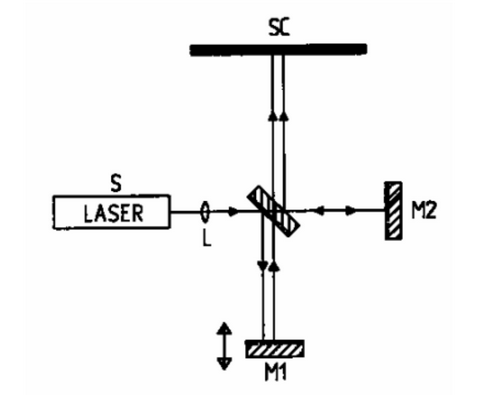
\includegraphics[height=5cm]{imagens/interferometer.png}
\small{\textit{\\Fonte: roteiro experimental.}}
\end{figure}

Como os dois feixes vieram da mesma fonte, as amplitudes e fases iniciais coincidem. Fazendo $I_1 = I_2$ na eq. \eqref{eq: interference formula}, temos
\begin{equation}
\begin{aligned}
\Delta = 2m\pi \implies I(\mathbf{r}) = 4I_1 \;, \\
\Delta = (2m+1)\pi \implies I(\mathbf{r}) = 0 \;.
\end{aligned}
\end{equation}

\noindent A diferença de fase nesse caso será apenas devido ao termo $\mathbf{k} \cdot (\mathbf{r}_2 - \mathbf{r}_1 ) = k_0 n d = 2\pi n d / \lambda_0$, onde $nd$ é a diferença de caminho óptico. 
Devido a periodicidade de $2\pi$ no padrão de interferência, ao contar um número inteiro $m$ de variação de mínimos ou máximos de interferência ao causar uma variação $nd$ no caminho óptico de um caminho em relação ao outro, a seguinte relação será verdadeira:
\begin{equation}
\frac{2\pi n d}{\lambda_0} = 2m\pi \implies \lambda_0 = \frac{nd}{m}.
\end{equation}


\section{Materiais e Métodos}

Lorem ipsum dolor sit amet, consectetur adipiscing elit. Nunc rhoncus, sapien sit amet finibus pulvinar, metus leo laoreet erat, a congue neque nulla sed felis. Maecenas ut luctus dui. In hac habitasse platea dictumst. Donec diam erat, facilisis sed nulla vitae, facilisis laoreet justo. Nunc fermentum magna purus, molestie sodales massa gravida varius. Phasellus id sagittis tellus. Nullam ullamcorper volutpat porttitor. In vestibulum diam ex. Integer lectus tortor, consequat interdum risus nec, commodo imperdiet ex. Sed euismod sagittis sapien, eget pellentesque risus aliquam quis. Proin lacinia dolor dui, quis facilisis urna volutpat ac.

\section{Resultados e Discussões}

\subsection*{Parte 1}

Os dados obtidos estão mostrados na tabela \ref{tab: exp1}. 
O valor médio encontrado para $\lambda$ foi $\langle \lambda \rangle = 633 \pm 26  \text{ nm} $, o que equivale a um desvio de 0,03$\%$ do valor informado pelo fabricante de 632,8 nm. Esse valor foi utilizado para os cálculo

\begin{table}[h]
\centering
\caption{Medidas do primeiro experimento.}
\begin{tabular}{c|c|c|c}
\toprule\midrule
$x_0$ (mm)& $x_1$ (mm) & $\Lambda$ ($\mu$m) & $\lambda$ (nm) \\
\midrule
0,45 & 0,62 & 34 & 567 \\
2,41 & 2,61 & 40 & 667 \\
7,13 & 7,32 & 38 & 633 \\
7,65 & 7,85 & 40 & 667 \\
9,21 & 9,40 & 38 & 633 \\
\midrule\bottomrule
\end{tabular}
\label{tab: exp1}
\end{table}

\subsection*{Parte 2}

Os dados obtidos estão mostrados na tabela \ref{tab: exp2}. Utilizando o software Grace para fazer uma regressão linear, mostrada na Fig. \ref{fig: regression}, foi encontrado o coeficiente linear $0,035479$ mbar$^{-1}$. Utilizando esse resultado na eq. \eqref{eq: kappa}, obtemos

\begin{equation*}
\begin{aligned}
\kappa &= \frac{(633 \times 10^{-9} \text{ m})}{2(4,1 \times 10^{-2} \text{ m})} (0,035470 \times 10^{3} \text{ mbar}^{-1}) \\ 
&= 2,74 \times 10^{-4} \text{ bar}^{-1}\;.
\end{aligned}
\end{equation*}

\begin{table}[b]
\centering
\caption{Dados do segundo experimento. Os valores da primeira coluna são adimensionais, os outros estão em mbar.}
\begin{tabular}{ccccccccccccc}
\toprule\midrule
$m$ & $P_{1}$ & $P_{2}$ & $P_{3}$ & $P_{4}$ & $P_{5}$ & $P_{6}$ & $P_{7}$ & $P_{8}$ & $P_{9}$ & $P_{10}$ & $\langle P \rangle$ & $\Delta P$\\
\midrule
5 & 220 & 220 & 200 & 220 & 210 & 220 & 200 & 220 & 220 & 220 & 215 & 7 \\
10 & 380 & 380 & 360 & 370 & 380 & 380 & 360 & 380 & 380 & 380 & 375 & 7 \\
15 & 540 & 540 & 520 & 520 & 520 & 520 & 500 & 530 & 540 & 530 & 526 & 10 \\
20 & 680 & 680 & 650 & 660 & 660 & 660 & 640 & 670 & 680 & 680 & 666 & 12 \\
25 & 780 & 770 & 780 & 780 & 760 & 760 & 740 & 780 & 780 & 770 & 770 & 10 \\
\midrule\bottomrule
\end{tabular}
\label{tab: exp2}
\end{table}

\noindent Tendo obtido $\kappa$, basta fazer $p = 1 \text{ bar}$ na eq. \eqref{eq: n(p)} para obter o valor de $n_{ar}$ à pressão atmosférica:

\begin{equation*}
\begin{aligned}
n_{ar} &= 1 + (2,74 \times 10^{-4} \text{ bar}^{-1})(1 \text{ bar}) \\
&= 1,000274 \;,
\end{aligned}
\end{equation*}

\noindent o que está de acordo com o valor informado pela literatura, de 1,000273 \ccite{wiki}, com um desvio percentual $<0,0001 \%$.

\begin{figure}[t]
\centering
\caption{Regressão linear dos dados do experimento 2. }
\includegraphics[width=0.8\columnwidth]{imagens/regression.eps}
\small{\\Fonte: Autor, 2026.}
\label{fig: regression}
\end{figure}


\begin{table}[h]
\centering
\caption{Medidas do terceiro experimento.}
\begin{tabular}{c|c|c}
\toprule\midrule
$m$ & $\theta$ ($^\circ$) & $n$ \\
\midrule   
40 & 6.7 & 1.8592 \\ 
40 & 6.8 & 1.8135 \\ 
60 & 8.8 & 1.6695 \\ 
60 & 8.6 & 1.7243 \\ 
60 & 8.4 & 1.7872 \\ 
60 & 8.6 & 1.7243 \\    
\midrule\bottomrule
\end{tabular}
\label{tab: exp3}
\end{table}

\subsection*{Parte 3}

Os dados obtidos estão mostrados na tabela \ref{tab: exp3}. O valor médio encontrado para $n$ foi $\langle n \rangle = 1,76 \pm 0,06$, que está no limite da faixa de valores dada pela literatura (entre 1,4 e 1,8).





\section{Conclusão}

Nesse trabalho, conseguimos determinar com alta precisão o valor do comprimento de onda do laser de HeNe e o índice de refração do ar em CNTP. Também conseguimos encontrar um valor para o índice de refração do vidro que é condizente com os valores conhecidos para outros vidros. Concluímos então que a interferometria é um método eficaz para fazer medidas precisas. Em particular, o interferômetro de Michelson é uma montagem relativamente simples e pode ser usada para fazer diversas medidas ópticas. 


%%%%%%% REFERENCIAS %%%%%%%%%
\begin{thebibliography}{10}
%Em chaves está o nome que será chamado durante o texto para citar a referência.


\end{thebibliography}


\end{document}
